\documentclass[journal]{IEEEtran}

\usepackage{times}
\usepackage{bm,bbm}
\usepackage{amsmath,amssymb}
\usepackage{graphicx,subfigure}
\usepackage{url}
\usepackage{siunitx}
\usepackage{cite,balance}
\usepackage{comment}
\usepackage{multirow}
\usepackage{booktabs}
\usepackage{microtype}
\usepackage{color}
\usepackage{rotating}

\def\citepunct{,\,}

\usepackage[normalem]{ulem} %%%% para tachar texto

\newtheorem{definition}{Definition}
\newtheorem{proposition}{Proposition}
\newcommand{\at}[2][]{#1|_{#2}}
\DeclareMathOperator*{\argmin}{arg\,min}

\begin{document}

%\title{SAR image classification using non parametric estimators of Shannon entropy}
\title{Entropy Estimators in SAR Image Classification}
\author{Julia~Cassetti, Daiana Delgadino, Andrea Rey and Alejandro~C.~Frery,~\IEEEmembership{Senior Member}
	
	%\thanks{This work was supported by Secretar\'ia de Pol\'iticas Universitarias (SPU), CNPq, and Fapeal.}
	
	\thanks{Julia Cassetti \texttt{jcassetti@campus.ungs.edu.ar} and Daiana Delgadino \texttt{ddelgadino@campus.ungs.edu.ar} are with the  Instituto de Desarrollo Humano, Universidad Nacional de General Sarmiento, Pcia. de Buenos Aires, Argentina.}
	\thanks{Andrea Rey \texttt{arey@frba.utn.edu.ar } is with Mathematics Department and Centro de Procesamiento de Señales e Imágenes, Universidad Tecnológica Nacional Facultad Regional Buenos Aires, Argentina.}
	
	\thanks{Alejandro C.\ Frery \texttt{alejandro.frery@vuw.ac.nz} is with the School of Mathematics and Statistics, Victoria University of Wellington, New Zealand.} 
}

\maketitle

\begin{abstract}
	
	Remotely sensed data are successfully used for information extraction. 
	In particular, SAR imagery, which suffers from speckle noise, needs unique models and techniques. 
	In this sense, the $\mathcal G^0$ family of distributions is a suitable model for SAR intensity because it can characterize areas with different degrees of texture. 
	Information theory has gained a place in signal and image processing for parameter estimation and feature extraction.
	Among its tools, entropy stands out as one of the most expressive features.
	This paper evaluates the performance of several parametric and nonparametric Shannon entropy estimators as input for supervised and unsupervised classification algorithms.
	Finally, we apply these methodologies to actual data.
	
\end{abstract}

\begin{IEEEkeywords}
	Feature extraction, synthetic aperture radar, Shannon entropy estimator, classification.
\end{IEEEkeywords}

\IEEEpeerreviewmaketitle

\section{Introduction}
\label{intro}
\IEEEPARstart{I}{mages} obtained with coherent illumination systems, such as Synthetic Aperture Radar (SAR), are contaminated by speckle. 
This noise-like interference phenomenon corrupts the image making it difficult to analyze and interpret. 

Under this perspective, statistical procedures are essential tools for processing SAR data. 
A suitable model to describe this sort of image is a fundamental point to obtain features that promote a good analysis. 
In this sense, the family of distributions $\mathcal{G}^0$~\cite{Frery97} has been extensively used to model SAR data because of its ability to a wide variety of roughness targets. 

Several approaches have been developed in order to obtain expressive and tractable features. 
In particular, entropy measures have been widely used for this purpose. 
Estimation parameter~\cite{gambini2015}, classification~\cite{Carvalho2019}, methodologies for constructing
confidence interval and contrast measures~\cite{Frery2012,Nascimento2009}, and edge detection~\cite{Nascimento2014} are some examples of its application.

Sundry authors have tackled the segmentation and classification SAR images problem using information theory measures. 
Nobre et al.~\cite{Nobre2016} used Rényi's entropy for monopolarized SAR image segmentation.
Ferreira et al.~\cite{Ferreira2020} derived a closed-form expression for the Shannon entropy based on the $\mathcal{G}^0$ law for intensity data and proposed a new entropy-based segmentation method. 
Carvalho et al.~\cite{Carvalho2019} employed stochastic distances to approach unsupervised classification methodology applied to Polarimetric Synthetic Aperture Radar (PolSAR) images. Palacio et al.~\cite{Palacio2019} used machine learning techniques in combination with filters to perform classification in PolSAR images.

The Shannon entropy has been applied to analyzed SAR imagery in several approaches, from inference~\cite{Frery2012} to classification~\cite{Ferreira2020}. 
Therefore, its estimation deserves attention. 
Vasicek~\cite{Vasicek76} replaced the distribution function $F$ by the empirical distribution function $F_n$ and used a difference operator in place of the differential operator in the Shannon entropy expression. 
Van Es~\cite{VanEs92} studied an entropy estimator based on differences between order statistics. 
Correa~\cite{Correa95} proposed a new entropy estimator determined from local linear regression.
Al-Omari~\cite{AlOmari2016} and Noughabi and Noughabi~\cite{Noughabi13} presented modified versions of the estimator introduced by Ebrahimi \emph{et al.}~\cite{Ebrahimi94}.

This paper addresses the classification problem through supervised and unsupervised strategies whose input is local entropy estimation. 
To this aim, we evaluate entropy estimators in both cases, parametric and nonparametric. 
In the parametric case, we use the relationship between $\mathcal{G}^0$ and Fisher distributions to obtain an expression of the entropy. 
In the nonparametric case, we assess these estimators in terms of bias, mean square error, computational time, and accuracy. 

\section{The $\mathcal{G}^0$ Model}
\label{sec_SAR}

The multiplicative model defines the return $Z$ in a monopolarized SAR image as the product of two independent random variables: one corresponding to the backscatter $X$, and the other to the speckle noise $Y$.
In this manner, $Z=X Y$ represents the return in each pixel of the image.

The $\mathcal{G}^{0}$ distribution family becomes attractive because of its flexibility to adequately model areas with all types of roughness~\cite{MejailJacoboFreryBustos:IJRS,  mejailfreryjacobobustos2001}. 
For intensity SAR data, this family arises from considering the speckle noise $Y$ modeled as a $\Gamma$ distributed random variable with unitary mean and shape parameter $L\geq1$, the number of looks. We also assume that the backscatter $X$ obeys a Reciprocal Gamma law.  
Thus, the density function for intensity data is given by
\begin{equation}
	f(z) =\frac{L^{L}\Gamma ( L-\alpha
		) }{\gamma ^{\alpha }\Gamma ( -\alpha ) \Gamma (
		L) }\cdot  
	\frac{z^{L-1}}{( \gamma +zL) ^{L-\alpha }},%
	\label{}
\end{equation}
where $-\alpha,\gamma ,z>0$ and $L\geq 1$. 
The $r$-order moment is
\begin{equation}
	\text{E}(Z^r) =\Big(\frac{\gamma}{L}\Big)^r\frac{\Gamma ( -\alpha-r )}{ \Gamma (-\alpha) } \cdot
	\frac{\Gamma (L+r )}{\Gamma (L)},
	\label{moments_gI0}
\end{equation}
provided $\alpha<-r$, and infinite otherwise.

Mejail et al.~\cite{MejailJacoboFreryBustos:IJRS} proved a relationship between $\mathcal G^0$ distribution and the Fisher-Snedekor $F$ law, which states that the cumulative distribution function $F_{\alpha,\gamma,L}$ for the return $Z$ is
\begin{equation}
	F_{\alpha,\gamma,L}(z) = \Upsilon_{2L, -2\alpha}(-\alpha  z / \gamma),
	\label{eq:CDFG0}
\end{equation}
for every $z>0$, where $\Upsilon_{2L, -2\alpha}$ is the cumulative distribution function of a Fisher-Snedekor random variable with $2L$ and $-2\alpha$ degrees of freedom.
This connection is helpful to obtain a closed formula for the entropy. 

\section{Shannon entropy}

%%% ACF Usar la notación usual para entropía: H
It is well known Shannon's contribution to the creation of what is known as Information Theory. 
Shannon~\cite{Shannon1948} proposed a new way of
measuring the transmission of information through a channel, thinking information as a statistical concept. 
In this regard, Shanon entropy (SE) is defined as
\begin{align}
	\label{SE}
	H[f(x)]&=-E[\log f(x)]=-\int_{-\infty}^{\infty} f(x) \log f(x) d x,
\end{align}
where $X$ is a continuous random variable with probability density function (pdf) $f(x)$ and
cumulative distribution function $F(x)$. 
The entropy of the~$\mathcal{G}^0$ distribution can be obtained using~\eqref{eq:CDFG0}.
Denote $H_{F}$ the entropy under the $F$ model, then the $\mathcal{G}^0$ entropy for intensity data $H_{\mathcal G^0}$ is 
\begin{align}
	\label{EntropiaFisherGi0}
	H_{\mathcal G^0}(\alpha,\gamma,L)=H_{F}(2 L, - 2 \alpha) -\log(-\alpha / \gamma).
\end{align}
Using~\eqref{EntropiaFisherGi0}, the
%%% Por qué "an"? Hay otras? Revisar todo.
expression of $H_{\mathcal G^0}$ is
\begin{align}
	\label{EG0}
	H_{\mathcal G^0}(\alpha,\gamma,L)&=-\log (-\alpha / \gamma)-(1-\alpha ) \psi^{(0)}(-\alpha )\\ \nonumber
	&+\log (-\alpha / L)+ ( L- \alpha ) \psi ^{(0)} ( L- \alpha )\\ \nonumber
	&+\log \big(B(L,-\alpha )\big)+(1-L) \psi^{(0)}(L),
\end{align}
where $\psi^{(0)}$ and $B$ are the digamma and beta functions, respectively.
%%% ACF Sería interesante graficar la entropía para a y g variando, con L fijo


%	\begin{figure}[hbt]
%		\centering    
%		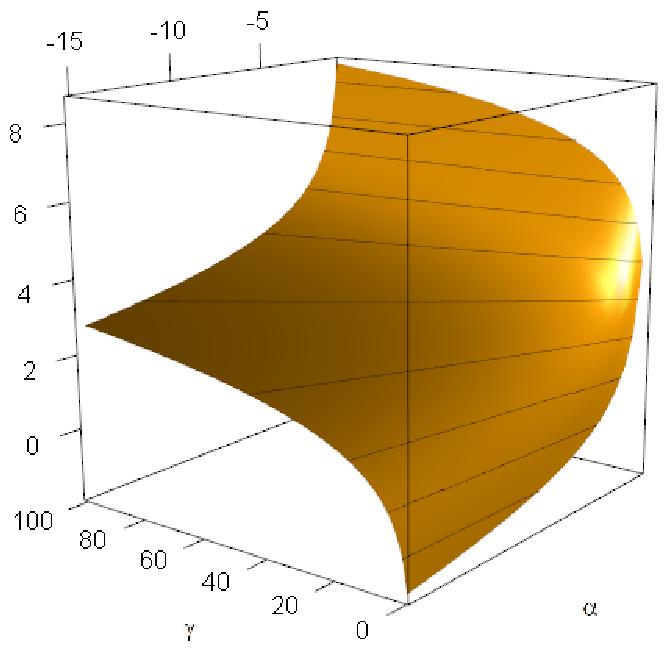
\includegraphics[width=0.6\linewidth]{../../../Figures/CISS2021/HG0L=3_2_2.pdf}
%		\caption{$H_{\mathcal G^0}(\alpha,\gamma,L)$ as a function of alpha and gamma for $L=2$.\label{figure:HG0}}
%	\end{figure}

\begin{figure}[hbt]
	\centering    
	\includegraphics[width=0.8\linewidth]{../../../Figures/CISS2021/entropiaL2.png}
	\caption{$H_{\mathcal G^0}(\alpha,\gamma,L)$ as a function of alpha and gamma for $L=2$.\label{figure:HG0}}
\end{figure}

%%% JC Hay dos programas GraficoEntropiaGI0_Figura1.R y Plot 3d H_Figura1.R

Figure~\ref{figure:HG0} shows the $H_{\mathcal G^0}(\alpha,\gamma,L)$ theoretical entropy as a function of $\alpha$ and $\gamma$ with $L=2$. 
It can be shown that for each fixed $\gamma$ value, $H_{\mathcal G^0}$ is an injective function. The same behavior repeats if we consider $\alpha$ as a constant.

\section{Shannon Entropy Estimators}

Several authors have proposed entropy estimators according to~\eqref{SE}.
Most of them are based on order statistics of the sample. 
Al-Omari~\cite{AlOmari2016} presented an overview of these estimators and also proposed a new one. 
From a parametric point of view, is natural to consider the maximum likelihood estimator (ML) of the entropy ($H_{\text{ML}}$).

In what follows, we describe the entropy estimators studied in this paper.

\subsection{Maximum likelihood entropy estimator}

Let $Z_1,\dots, Z_n$ be an independent random sample of size $n$ from the $\mathcal G^0(\alpha,\gamma,L)$ distribution.
Assume $L$ is known.
The maximum likelihood estimator of $\alpha$ and $\gamma$ for $L$ known, denoted $\widehat\alpha_{\text{ML}}$ and $\widehat\gamma_{\text{ML}}$ respectively, consists of the values in the parametric space $\mathbbm R_-\times\mathbbm R_+$, that maximize the loglikelihood function:
\begin{multline}
	\log \Gamma(L-\widehat\alpha_{\text{ML}})-
	\widehat\alpha_{\text{ML}}\log \widehat\gamma_{\text{ML}} -\log\Gamma(-\widehat\alpha_{\text{ML}})  \\
	\mbox{}+\frac{\widehat\alpha_{\text{ML}}-L}{n} \sum_{i=1}^n\log\big(\widehat\gamma_{\text{ML}}+L Z_i\big).
	\label{ML}
\end{multline}
Optimal asymptotic properties of the ML estimator are well-known and its calculation demands numerical maximization routines.
We use the L-BFGS-B version of the Broyden-Fletcher-Goldfarb-Shanno (BFGS) method~\cite{Luenberger2008} that allows box constraints.
This algorithm belongs to the quasi-Newton methods family, not requiring the Hessian matrix but only the gradient.

The ML entropy estimator~\cite{CaseBerg01} is
\begin{align}
	H_\text{ML}=H_{\mathcal G^0}(\widehat{\alpha}_{\text{ML}},\widehat{\gamma}_{\text{ML}},L).
\end{align}

%; the left-hand-side of~\eqref{rootML} is the gradient of~\eqref{ML}. 

%Function~\eqref{ML} is, in general, unimodal but, depending on the sample, it may be monotonically decreasing. 
%This behavior is the responsible for the algorithm failing to converge.


\subsection{Non-parametric entropy estimators}
\label{Hest}

The problem of estimating entropy has attracted the interest of several authors. For continuous random variables Vasicek~\cite{Vasicek76} showed that the functional defined in~\eqref{SE} can be written as
\begin{align}
	H[f(x)]=\int_{0}^{1} \log \frac{d F^{-1}(p)}{d p} d p,
\end{align}
considering the change of variables $x=F^{-1}(p).$
He proposed to estimate the cumulative distribution function  $F(X)$ with the empirical cumulative distribution function $F_n(x)$ and used the difference operator instead of the differential operator in order to approximate ${d F^{-1}(p)}/{d p}$ by a function of the order statistics.

Assume $X_1,\dots,X_n$ is a random sample from the distribution function $F(x)$ whose order statistics are $X_{(1)}, \ldots, X_{(n)}$. 
Vasicek~\cite{Vasicek76} proposed the following entropy estimator,
\begin{align}
	\label{HV}
	H_{\text{V}}=\frac{1}{n} \sum_{i=1}^{n} \log \Big[\frac{n}{2 m}\big(X_{(i+m)}-X_{(i-m)}\big)\Big], 
\end{align}
with $m<n/2$ a positive integer number, $X_{(i+m)}-X_{(i-m)}$ the spacing of order $m$, or $m$-spacing, $X_{(i)}=X_{(i)}$ if $1<i$ and $X_{(i)}=X_{(n)}$ if $i>n$.
The author proves that this estimator is weakly consistent for $H(f)$ when $m/n \to 0$ and $n,m \to \infty$.

Several authors introduced modifications to the Vasicek estimator. In this work we also consider the following entropy estimators which were presented by Al-Omari~\cite{AlOmari2016}. 
%In the following we present the expression of the studied estimators. 
%It should be noted that most of the estimators studied in this work 
%%% ACF m y n van en modo matemático
%%% ACF citar los artículos originales
\begin{itemize}
	%%% ACF Qué es m?
	\item Van Es~\cite{VanEs92}:
	\begin{align}
		\label{HVE}
		H_\text{VE}&=\frac{1}{n-m} \sum_{i=1}^{n-m}\log{\Big[\frac{n+1}{m}\big(X_{(i+m)}-X_{(i)}\big)\Big]} \nonumber\\
		&+\sum_{k=m}^{n} \frac{1}{k}+\log \frac{m}{n+1}.
	\end{align}
	\item Correa~\cite{Correa95}:
	\begin{align}
		\label{HC}
		H_\text{C}=-\frac{1}{n} \sum_{i=1}^{n} \log \frac{\sum_{j=i-m}^{i+m}(j-i)\left(X_{(j)}-\overline{X}_{(i)}\right)}{n \sum_{j=i-m}^{i+m}\big(X_{(j)}-\overline{X}_{(i)}\big)^{2}},
	\end{align}
	where $\overline{X}_{(i)}=(2 m+1)^{-1} \sum_{j=i-m}^{i+m} X_{(j)}$.
	\item Noughabiet et al.~\cite{Noughabi2010} 
	\label{HNA}
	\begin{align}
		H_\text{NA}=\frac{1}{n} \sum_{i=1}^{n} \log \Big[\frac{n}{c_{i} m}\big(X_{(i+m)}-X_{(i-m)}\big)\Big]
	\end{align}
	where 
	\begin{equation*}
		c_{i}=\left\{\begin{array}{ll}
			1 & \text{ if }1 \leq i \leq m, \\
			2 & \text{ if }m+1 \leq i \leq n-m, \\
			1 & \text{ if }n-m+1 \leq i \leq n,
		\end{array}\right.
	\end{equation*}
	and $X_{(i-m)}=X_{(1)}$ if $i \leq m$ and $X_{(i+m)}=X_{(n)}$ for $i \geq n-m $. 
	\item Al-Omari~\cite{AlOmari2014}:
	\begin{align}
		H_{{\text{AO}}_1}=\frac{1}{n} \sum_{i=1}^{n} \log \Big[\frac{n}{\omega_{i} m}\left(X_{(i+m)}-X_{(i-m)}\right)\Big], 
		\label{AHE}
	\end{align}
	where
	\begin{equation*}
		\omega_{i}= \begin{cases}
			3/2 & \text{ if }1 \leq i \leq m, \\
			2 & \text{ if } m+1 \leq i \leq n-m, \\
			3/2 & \text{ if } n-m+1 \leq i \leq n,
		\end{cases}
	\end{equation*}
	in which $X_{(i-m)}=X_{(1)}$ for $i \leq m$, and $X_{(i+m)}=X_{(n)}$ for $i \geq n-m$. 
	
	\item Al-Omari alternative proposal~\cite{AlOmari2016}:
	\label{AO2}
	\begin{align}
		H_{{\text{AO}}_2}=\frac{1}{n} \sum_{i=1}^{n} \log \Big[\frac{n}{v_{i} m}\left(X_{(i+m)}-X_{(i-m)}\right)\Big],
	\end{align}
	where
	\begin{equation*}
		v_{i}=\begin{cases}
			1+(i-1)/m & \text{ if }1 \leq i \leq m, \\
			2 & \text{ if } m+1 \leq i \leq n-m, \\
			1+(n-i)/2m & \text{ if } n-m+1 \leq i \leq n,
		\end{cases}
	\end{equation*}
	in which $X_{(i-m)}=X_{(1)}$ for $i \leq m$, and $X_{(i+m)}=X_{(n)}$ for $i \geq n-m$.
	\item Ebrahimi~\cite{Ebrahimi94}
	\begin{align}
		H_\text{E}=\frac{1}{n} \sum_{i=1}^{n} \log \Big[\frac{n}{\tau_{i} m}\left(X_{(i+m)}-X_{(i-m)}\right)\Big],
		\label{HE}
	\end{align}
	where
	\begin{equation*}
		\tau_{i}=\begin{cases}
			1+(i-1)/m & \text{ if }1 \leq i \leq m, \\
			2 & \text{ if } m+1 \leq i \leq n-m, \\
			1+(n-i)/m & \text{ if } n-m+1 \leq i \leq n.
		\end{cases}
	\end{equation*}
\end{itemize}

Van Es~\cite{VanEs92} showed that, under general conditions, \eqref{HVE} converges almost surely to $H[f(x)]$ when $m, n \to \infty$, $m/\log(n) \to \infty$, and $m/n \to 0$.
The author also proved the estimator's asymptotic normality when $m, n \to \infty$ and $m = o(n^{1/2})$. 
Correa~\cite{Correa95}, through a simulated study, showed that his estimator has a smaller mean squared error than Vasiciek's  proposal~\eqref{HV}. 

Al-Omari\cite{AlOmari2014} presented three estimators based on different sampling methods.
In this paper we studied the simple random sampling one (\textit{SRS})~\eqref{AHE} and second proposal suggested
in \cite{AlOmari2016}. 
The author proved that these estimators converge in probability to $ H[f(x)]$ when $m, n \to \infty  \text{ and } m/n \to 0$. 
Ebrahimi et al~\cite{Ebrahimi94} presented an estimator adjusting the Vasicek's\cite{Vasicek76} weight. 
Under the same conditions than Al-Omari\cite{AlOmari2014} the authors proved that $H_{\text{E}}\underset{n \to \infty}{\overset{p}{\longrightarrow}} H[f(x)]$ when $m, n \to \infty  \text{ and } m/n \to 0$. 
The same applies to Noughabi et al. estimator~\cite{Noughabi2010}.

\section{Simulation study}\label{sec:simulation}

The choice of the spacing parameter $m$ in this kind of estimator is an important task that is still open. Wieczorkowski et al.~\cite{Wieczorkowski1999} proposed a heuristic formula $m=[\sqrt{n}+0.5]$. To assess the performance of this criterion, we conducted a Monte Carlo study for the entropy estimators presented in section~\ref{Hest} under the $\mathcal{G}^0$ model.

We generated $1000$ samples from a $\mathcal{G}^0$ distribution of size $n \in\left\lbrace 9,25,49,81,121\right\rbrace $ for each textured value $\alpha \in\left\lbrace -8,-5-3,-1.5\right\rbrace $ and $L=2$. For each non-parametric study we use the $m$ value chosen with the Wieczorkowski et al. proposal.
The sample sizes chosen represent different scenarios of window sizes. Since the parameter $\gamma$ is proportional to the brightness, meaning it is a scale parameter, we based the forthcoming analysis on the condition $E(Z)=1$, which links texture and brightness parameter by $\gamma^* =-\alpha-1$. 

Each replication produces a vector  of estimators $(\widehat{H}_1, \dots, \widehat{H}_{1000})$ from which we compute sample mean $\overline{\widehat{H}}$, 
sample bias $\widehat{B}=B_{\widehat{H}} = \overline{\widehat{H}}- H$ where $H$ is the true entropy value, and sample mean squared error (MSE) $\widehat{\textrm{MSE}}=({1000})^{-1}{\sum_{i=1}^{1000}{(\widehat{H}_i-H)^2}}$.

Figures~\ref{Sesgo_W_L=2} and~\ref{ECM_W_L=2} presented the bias and the MSE for the Wieczorkowski et al.~\cite{Wieczorkowski1999} criterion, $L=2$ case and for all of the estimators analyzed, except for Al-Omari~\eqref{AO2} and Ebrahimi~\eqref{HE} estimators due to the large bias they presented in the simulation study.  
\begin{figure}[hbt]
	\centering
	\subfigure[\label{Sesgo_W_L=2}Bias]{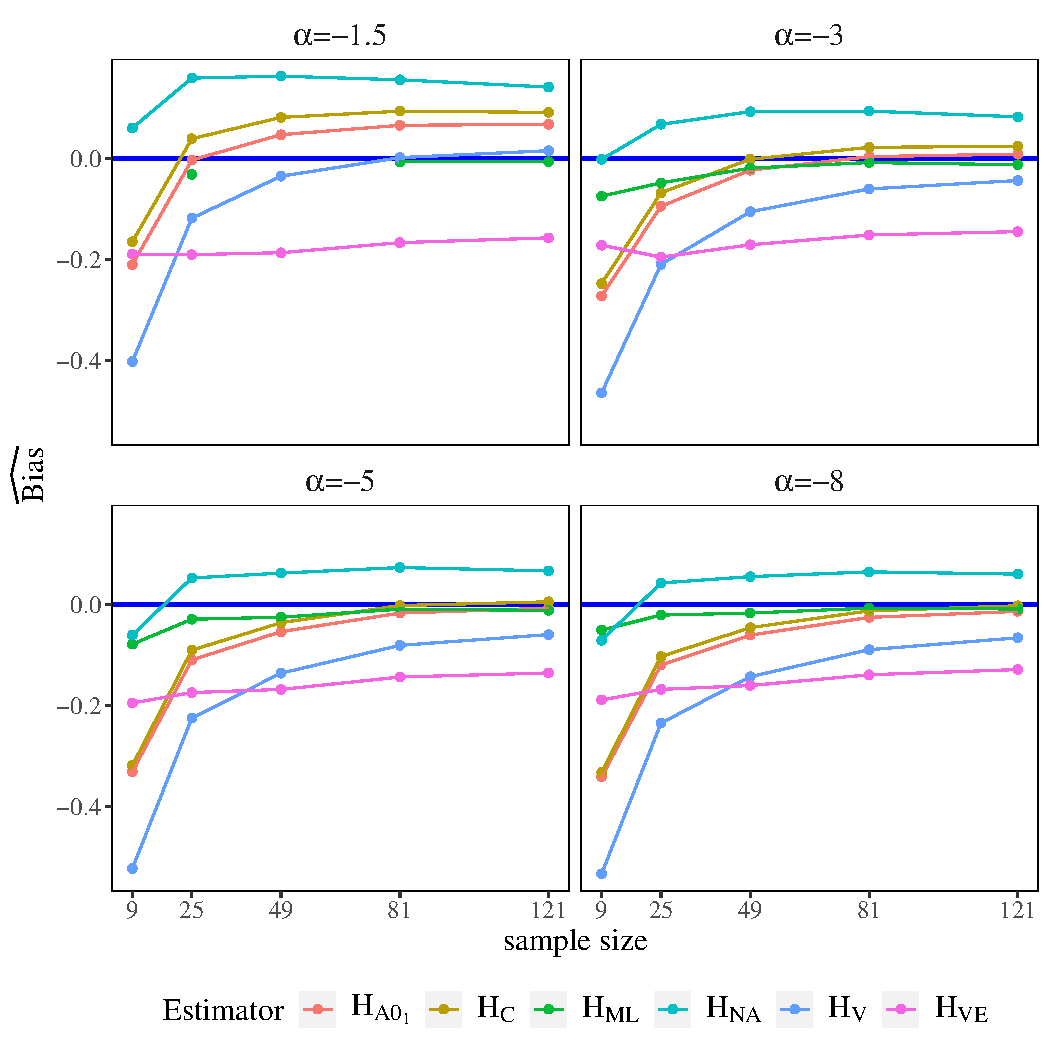
\includegraphics[width=\linewidth]{../../../Figures/CISS2021/Grafico_Hest_Sesgo_mW_L=2ConNeg}}
	\subfigure[\label{ECM_W_L=2}Mean Square Error]{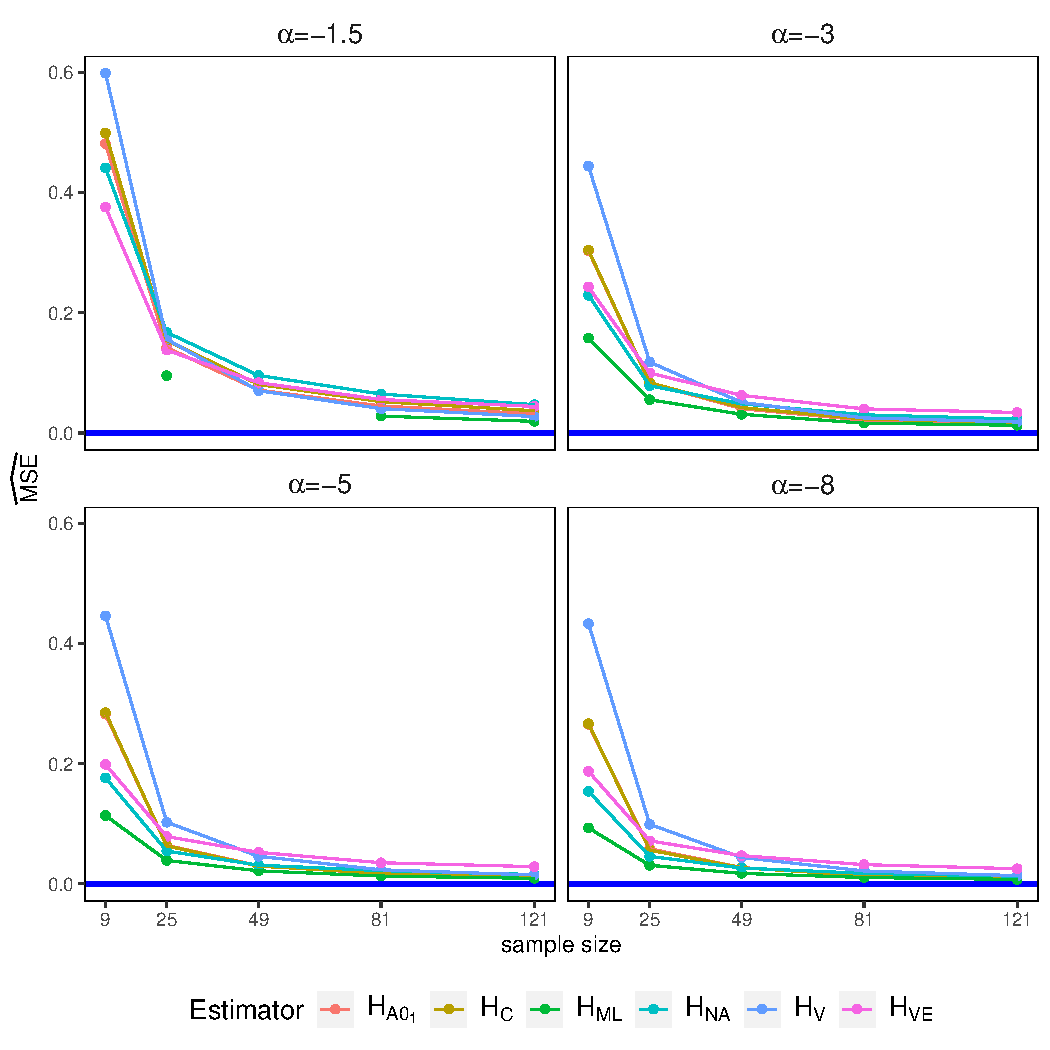
\includegraphics[width=\linewidth]{../../../Figures/CISS2021/Grafico_Hest_ECM_mW_L=2ConNeg}}
	\caption{Bias and MSE for Wieczorkowski criterion, $L=2$.}
\end{figure}    

%%% JC Figura2.Rmd
%%% ACF Editada

It can be seen that there is no single estimator that performs well for all $\alpha$ values. 
$H_\text{C}$ and $H_{\text{AO}_1}$ present low bias and low MSE for all the cases study except for $\alpha=-1.5$. 
The others estimators show bad behavior for all the cases studied.	

In order to improve the Wieczorkowski et al.~\cite{Wieczorkowski1999} criterion, we implement another strategy to choose, for each sample size $n$, the best $m$ value to be used for all $\alpha$ values.

Table~\ref{tab:eleccion_mejor_m} shows the schema of the methodology employed, for fixed $n$ value and entropy estimator. 
Each table entry, $\widehat{B}_{ij}$, represents the bias for $m=i$ and $\alpha \text{=} \alpha_j$. 
For each estimator and each fixed $m$ value we calculate the average bias ($\overline{\widehat{B}}$) between different $\alpha$ values. Finally, the chosen $m$ is the argument that minimizes the average bias.

\begin{table}[hbt]
	\caption{Selection criterion for the best $m$ for each $n$ and each entropy estimator, with $\alpha_1= -1.5$, $\alpha_2=-3$, $\alpha_3=-5$ and $\alpha_4=-8$.}
	\label{tab:eleccion_mejor_m}
	\centering
	\begin{tabular}{c c c c c c}
		\toprule
		$m$	& $\alpha_{1}$ & $\alpha_{2}$
		& $\alpha_{3}$
		& $\alpha_{4}$ & $\overline{\widehat{B}}$ \\
		
		\midrule
		$1$	& $\widehat{B}_{11}$ & $\widehat{B}_{12}$ & $\widehat{B}_{13}$ & $\widehat{B}_{14}$ & $\overline{\widehat{B}}_{1.}$\\
		
		$2$	& $\widehat{B}_{21}$ & $\widehat{B}_{22}$ & $\widehat{B}_{23}$ & $\widehat{B}_{24}$ & $\overline{\widehat{B}}_{2.}$\\
		$\vdots$ & $\vdots$ & $\vdots$ & $\vdots$ & $\vdots$ & $\vdots$ \\
		
		$i$ & $\widehat{B}_{i1}$ & $\widehat{B}_{i2}$ & $\widehat{B}_{i3}$ & $\widehat{B}_{i4}$ & $\overline{\widehat{B}}_{i.}$\\
		$\vdots$ & $\vdots$ & $\vdots$ & $\vdots$ & $\vdots$ & $\vdots$\\
		
		$\lfloor n/2 \rfloor$ & $\widehat{B}_{N1}$ & $\widehat{B}_{n2}$ & $\widehat{B}_{n3}$ & $\widehat{B}_{n4}$ & $\overline{\widehat{B}}_{n.}$\\
		\bottomrule
		& & & & & $m=\argmin\limits_{i} \overline{\widehat{B}}_{i}$\\
		
		\bottomrule
	\end{tabular}
\end{table}	

Table~\ref{tab:Mejor_m} shows the best $m$ chosen according to the methodology used for $L=1$ and $L=2$ respectively, for samples coming from $\mathcal{G}_0$ distribution. 

\begin{table}[htbp]
	\label{tab:Mejor_m}
	\centering
	\caption{Best $m$ chosen for each $n$ and entropy estimator.}
	\begin{tabular}{crcccrc}
		\toprule
		$L$     & \multicolumn{1}{l}{$n$} & \multicolumn{1}{l}{$H_{{\text{AO}}_1}$} & \multicolumn{1}{l}{$H_\text{C}$} & \multicolumn{1}{l}{$H_{\text{NA}}$} & \multicolumn{1}{l}{$H_\text{V}$} & \multicolumn{1}{l}{$H_{\text{VE}}$} \\
		\midrule
		\multirow{5}[1]{*}{1} 
		& $9$     & $4$     & $4$     & $3$     & $4$     & $4$ \\
		& $25$    & $6$     & $5$     & $3$     & $8$     & $2$ \\
		& $49$    & $7$     & $5$     & $4$     & $9$     & $2$ \\
		& $81$    & $7$     & $4$     & $5$     & $8$     & $2$ \\
		& $121$   & $9$     & $4$     & $6$     & $11$    & $2$ \\
		\midrule
		\multirow{5}[0]{*}{2} 
		& $9$     & $4$     & $4$     & $3$     & $3$     & $2$ \\
		& $25$    & $8$     & $4$     & $4$     & $9$     & $2$ \\
		& $49$    & $8$     & $4$     & $5$     & $9$     & $2$ \\
		& $81$    & $9$     & $4$     & $5$     & $9$     & $2$ \\
		& $121$   & $10$    & $5$     & $6$     & $10$    & $2$ \\
		\bottomrule
	\end{tabular}
\end{table}


Figures~\ref{Sesgo_HL=2ConNeg} and~\ref{ECM_HL=2ConNeg} show the behavior of the estimators studied for the $m$ value chosen in terms of bias and MSE respectively for $L=2$ case. We also plot the $H_{\text{ML}}$ estimator. It can be observed the improvement in entropy estimation in terms of bias and MSE with our methodology, compared with the Wieczorkowski et al. empirical formula for all of the estimators studied.

\begin{figure}[hbt]
	\centering
	\subfigure[\label{Sesgo_HL=2ConNeg}$\widehat{\text{Bias}}$]{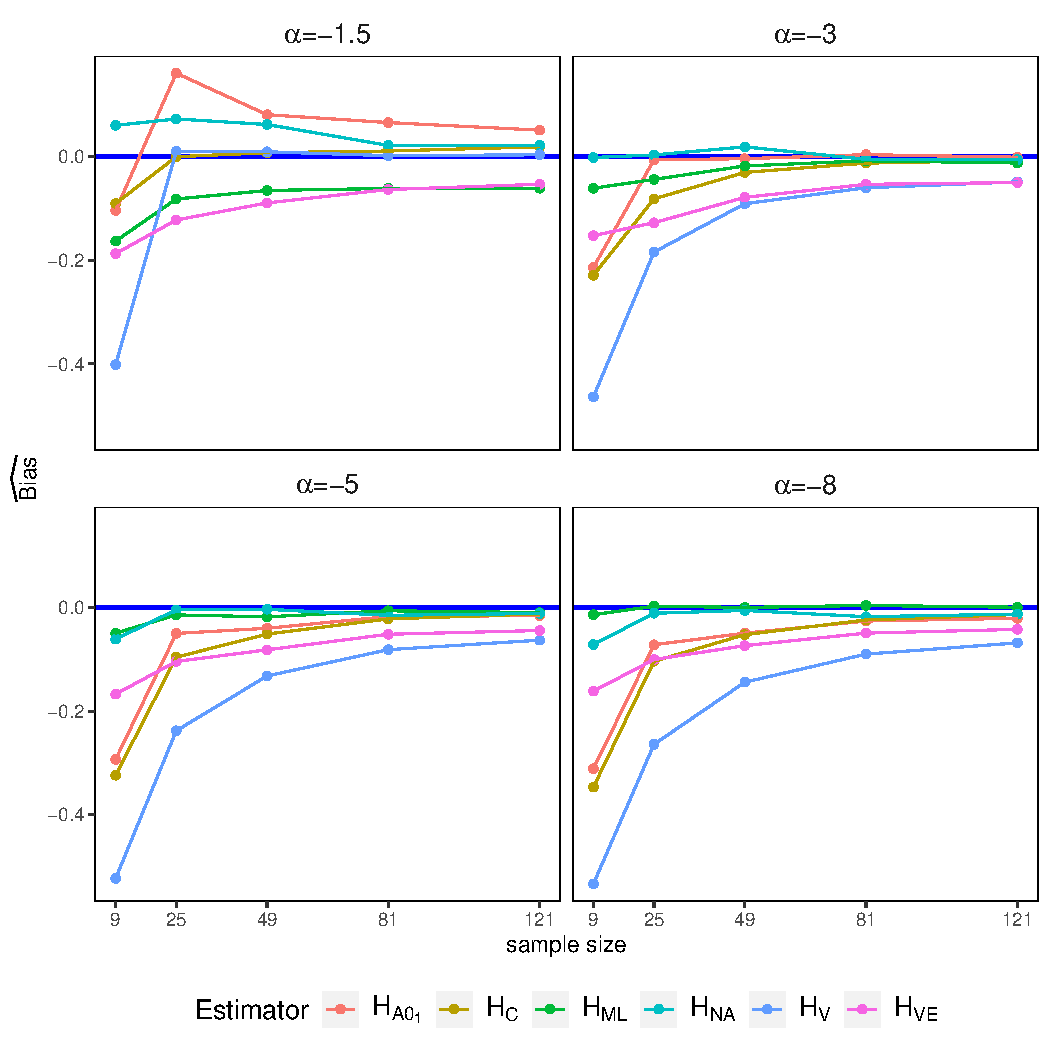
\includegraphics[width=\linewidth]{../../../Figures/CISS2021/Grafico_Hest_Sesgo_L=2ConNeg.pdf}}
	\subfigure[\label{ECM_HL=2ConNeg}$\widehat{\text{MSE}}$]{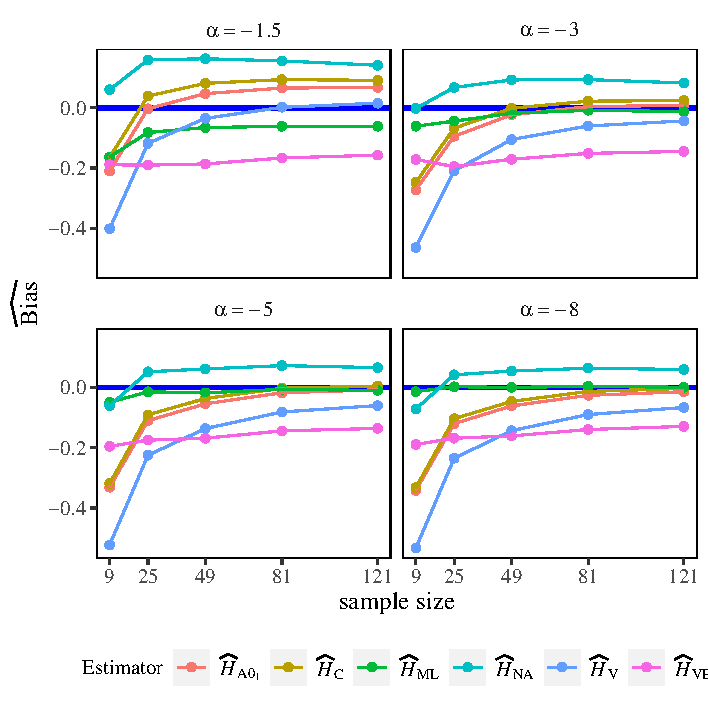
\includegraphics[width=\linewidth]{../../../Figures/CISS2021/Grafico_Hest_ECM_L=2ConNeg.pdf}}
	\caption{Bias and MSE for authors proposal $m$ choice, $L=2$.} 
\end{figure}     

%%% JC Figura3.Rmd
%%% ACF Editada

We continue studying the quality of these estimators in the SAR image classification framework.
%	We then assessed the performance of these estimators in the frame of supervised classification by applying the support vector machine (SVM) technique, and of unsupervised classification using $k$-means. 
%	With this purpose, we generated synthetic images varying the values of $\alpha$ and $\gamma$, and used sliding windows of different sizes to obtain the entropy map. 
%	The classifier used these maps as features. 
%	The classification methods were evaluated using Kappa coefficient and overall accuracy. 
%	Moreover, the parameter estimation methods were tested in actual SAR data. 

%	The details and results will be presented in the final paper.

\section{Classification}
\label{Classification}

To study the performance of the selected entropy estimators in terms of  SAR image classification, we divided the analysis into simulated and actual images. 
We used unsupervised and supervised techniques to choose the three best estimators that present the best values of classification quality. 
For the former, we carried out a $k$-means algorithm, which groups data into $k$ classes setting $k$ centroids and minimizing the variance within each group. 
This nonhierarchical clustering technique is applied in many studies in SAR image processing. 
Niharika et al.~\cite{Niharika2017} put forward a segmentation algorithm for SAR images based on $k$-means classification and thresholding techniques. 
Liu et al.~\cite{Liu2019} propose a $k$-means clustering technique for SAR image change detection.

For the latter approach we implemented a support vector machine (SVM) algorithm, which is a supervised machine learning technique based on the statistical learning theory~\cite{Vapnik1995} whose objective is to define, given a set of features,  the best possible separation between classes by finding a hyperplane that maximizes the margin of separation between these classes. It is common to sacrifice some misclassification to get a better overall performance, introducing a penalizing parameter $c$. When data cannot be separated by a hyperplane, they are transformed to a higher dimensional feature space through a suitable nonlinear transformation called kernel function. Given $\textrm{\textbf{x}}, \textrm{\textbf{x'}} \in \mathbb{R}^n$, linear and radial kernels are respectively defined by $K_L(\textrm{\textbf{x}}, \textrm{\textbf{x'}})=\langle \textrm{\textbf{x}}, \textrm{\textbf{x'}} \rangle$ and $K_R(\textrm{\textbf{x}}, \textrm{\textbf{x'}})=\exp(-g\lVert \textrm{\textbf{x}}-\textrm{\textbf{x'}} \rVert^2)$, for $g>0$.

This method has been widely applied in different areas such as sea oil spill monitoring~\cite{Fan2015}, pattern recognition~\cite{svmtutorialBURGES1999}, classification of polarimetric SAR Image~\cite{Palacio2019,Zhang2010} among other applications.

To measure the quality of these algorithms, we use different measures depending on the type of classification. For example, in the unsupervised case, we use Calinski-Harabasz (CH)~\cite{Calinski1974} and Davies-Bouldin~\cite{Davies1979} (DB) indexes,  Kappa coefficients for the supervised classification and accuracy for both algorithms. 

In the following, we present empirical results classifying a simulated image SAR.

%The former is defined as
%\begin{equation}
%\label{CH}
%CH=\frac{S S_{B}}{S S_{W}} \times \frac{N-k}{k-1}
%\end{equation}
%where $\mathrm{k}$ is the number of clusters, $\mathrm{N}$ is the total number of %observations (data points), $S S_{W}$ is the total within sum of squares and $S S_{B}$ is %the overall total between sum of squares. The latter is defined as

%\begin{equation}
%\label{DB}
%DB=\frac{1}{k} \sum_{i=1, i \neq j}^{k} \max \left(\frac{S_{i}+\S_{j}}{d\left(c_{i}, %c_{j}\right)}\right)
%\end{equation}
%where $\mathrm{k}$ is the number of clusters, $S_{i}$ ($S_{j}$) is the average distance %between each point in cluster $i$ (cluster $j$ respectively) and the centroid of the %cluster, and $d\left(c_{i}, c_{j}\right)$ is the distance between the centroids of both %cluster.

\subsection{Simulated image}
\label{sec:synthetic}

Figure~\ref{fig:syntheticL2} shows a $300 \times 300$ image generated with a $\mathcal{G}^0$ distribution with $L=2$, $\gamma=0.1$ and four different classes according to the value of $\alpha \in \{-1.5, -3, -5 -8\}$. The light gray level corresponds to an extremely textured area corresponding to the value $\alpha=-1.5$. As the gray level decreases, the texture of the zone changes from heterogeneous ($\alpha=-3$ and $-5$) to a homogeneous zone corresponding to the darkest gray level ($\alpha=-8$). 

\begin{figure}[hbt]
	\centering
	\subfigure[\label{fig:syntheticL2} Simulated image]{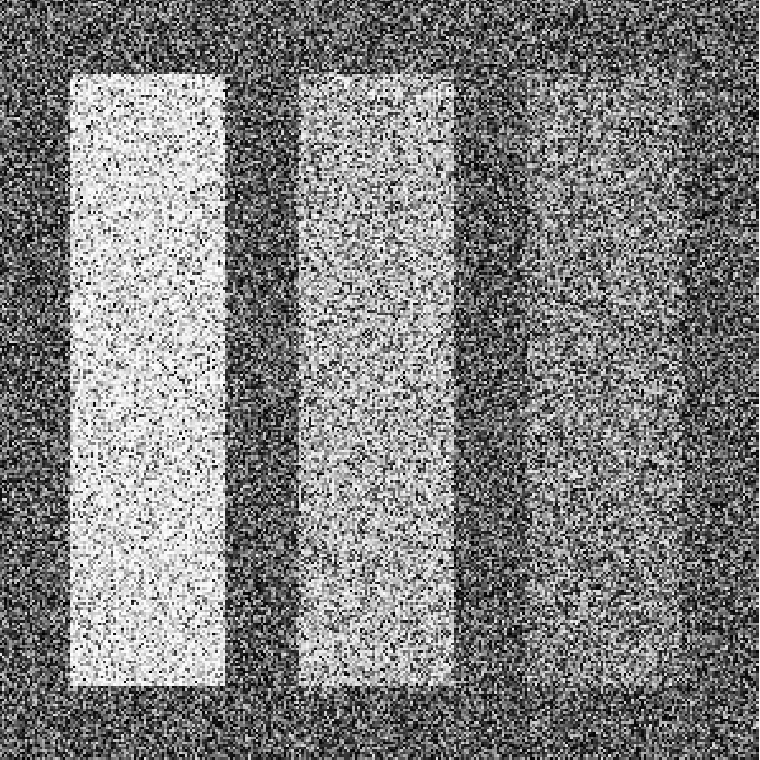
\includegraphics[width=0.49\linewidth]{../../../Figures/CISS2021/SinteticaL2.pdf}}
	\subfigure[\label{fig:kmeansHCL2}$K$-means $H_\text{C}$ estimator]{\includegraphics[width=0.49\linewidth]{../../../Figures/CISS2021/kmeansHC_SyntheticL2.pdf}}
	\subfigure[\label{fig:AccuracyL2}Accuracy]{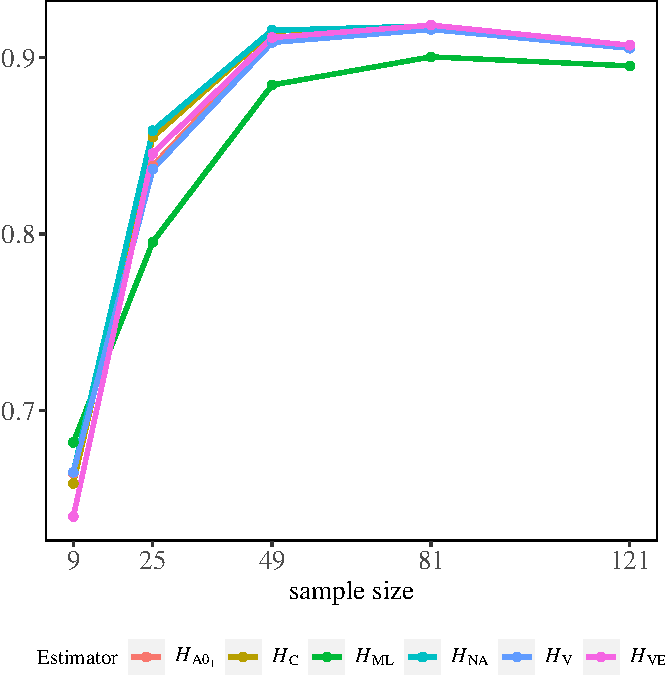
\includegraphics[width=.8\linewidth]{../../../Figures/CISS2021/Accuracy_L2.pdf}}
	\caption{$K$-means applied to a simulated image with $L=2$, $\gamma=0.1$ and  sliding windows size $9 \times 9$.} 
\end{figure}  

%%% JC GraficoAccuracyL2_Figura4.R
%%% ACF Editada

For each estimator we perform a map of estimated entropies ($\widehat{H}$) by sweeping the image with sliding windows of sizes $s\times s$, for $s=3,5,7,9,11$, corresponding to the sample sizes studied in section~\ref{sec:simulation}. Then, we use $\widehat{H}$ as a feature to classify by both the unsupervised and supervised techniques.

For each windows size we applied $k$-means algorithm to the simulated image. Figure~\ref{fig:AccuracyL2} shows the accuracy according to the chosen sample size. It can be observed that a $9 \times 9$ window presents the best value of accuracy. It can also be seen that the $H_{\text{ML}}$ estimator presents the worth performance whereas $H_\text{C}$, $H_{\text{NA}}$ and $H_{\text{VE}}$ show the best performance, as is indicated in Table~\ref{tab:accuracy} with bold letter. Figure~\ref{fig:kmeansHCL2} shows the result of applied a $k$-means classification for $H_\text{C}$ estimator. Table~\ref{tab:CHyDB_synt} presents the value of CH and DB indexes for $n=81$ sample size. It can be observe that for the former case, $H_\text{C}$, $H_{\text{NA}}$ and $H_{\text{VE}}$ estimators have the best performance, and for the latter $H_\text{C}$, $H_{\text{NA}}$ and $H_{\text{V}}$ were the best.

\begin{table}[htbp]
	\centering
	%\caption{Measures index for synthetic image}
	\caption{Accuracy for $k$-means ($k=4$) applied to simulated data}
	\label{tab:accuracy}
	\begin{tabular}{crrrrrr}
		%\multicolumn{7}{c}{Accuracy} \\
		\midrule
		$n$     & \multicolumn{1}{c}{$H_{{\text{AO}}_1}$} & \multicolumn{1}{c}{$H_\text{C}$} & \multicolumn{1}{c}{$H_{\text{NA}}$} & \multicolumn{1}{c}{$H_\text{V}$} & \multicolumn{1}{c}{$H_{\text{VE}}$} & \multicolumn{1}{c}{$H_{\text{ML}}$}\\
		\midrule
		9 & 0.664 & 0.659 & 0.665 & 0.665 & 0.640 & 0.682 \\
		25  & 0.839 & 0.855 & 0.859 & 0.837 & 0.846 & 0.796 \\
		49  & 0.911 & 0.915 & 0.915 & 0.909 & 0.911 & 0.884 \\
		81  & 0.916 & \textbf{0.918} & \textbf{0.918} & 0.916 & $\textbf{0.918}$ & 0.900 \\
		121 & 0.905 & 0.906 & 0.907 & 0.905 & 0.907 & 0.895 \\
		\bottomrule
	\end{tabular}%
	\label{tab:addlabel}%
\end{table}

\begin{table}[htbp]
	\centering
	\caption{Classification quality indexes for $k$-means ($k=4$) applied to simulated data with $n=81$}
	\label{tab:CHyDB_synt}
	\begin{tabular}{crrrrrr}
		%\multicolumn{8}{c}{Indexes} \\
		\midrule
		Index   & $H_{{\text{AO}}_1}$ & \multicolumn{1}{c}{$H_\text{C}$} & \multicolumn{1}{c}{$H_{\text{NA}}$} & \multicolumn{1}{c}{$H_\text{V}$} & \multicolumn{1}{c}{$H_{\text{VE}}$} & \multicolumn{1}{c}{$H_{\text{ML}}$} \\
		\midrule
		CH	&	852914	&	\textbf{898079}	&	\textbf{902719}	&	852914	&	\textbf{867746}	&	703774	\\
		DB	&	0.441	&	\textbf{0.434}	&	\textbf{0.433}	&	\textbf{0.441}	&	0.442	&	0.467	\\
		
		\midrule
		
	\end{tabular}%
	\label{tab:addlabel}
\end{table}%

%\begin{table}[htbp]
%  \centering
%  \caption{Measures index for synthetic image}
%  \label{tab:measures_synt}
%    \begin{tabular}{crrrrrr}
%     \multicolumn{7}{c}{Accuracy} \\
%    \midrule
%    $n$     & \multicolumn{1}{c}{$H_{{AO}_1}$} & \multicolumn{1}{c}{$H_\text{C}$} & %\multicolumn{1}{c}{$H_{\text{NA}}$} & \multicolumn{1}{c}{$H_\text{V}$} & \multicolumn{1}{c}{$H_{\text{VE}}$} & %\multicolumn{1}{c}{$H_{\text{ML}}$} \\
%    \midrule
%    $9$ & $0.664$ & $0.659$ & $0.665$ & $0.665$ & $0.640$ & $0.682$ \\
%    $25$  & $0.839$ & $0.855$ & $0.859$ & $0.837$ & $0.846$ & $0.796$ \\
%    $49$  & $0.911$ & $0.915$ & $0.915$ & $0.909$ & $0.911$ & $0.884$ \\
%    $81$  & $0.916$ & \textcolor{red}{$0.918$} & \textcolor{red}{$0.918$} & $0.916$ & %\textcolor{red}{$0.918$} & $0.900$ \\
%    $121$ & $0.905$ & $0.906$ & $0.907$ & $0.905$ & $0.907$ & $0.895$ \\
%    \midrule
%     &       &       &       &       &       &  \\
%
%    \multicolumn{7}{c}{Calinski-Harabasz} \\
%    \midrule
%    $n$     & \multicolumn{1}{c}{$H_{{AO}_1}$} & \multicolumn{1}{c}{$H_\text{C}$} & %\multicolumn{1}{c}{$H_{\text{NA}}$} & \multicolumn{1}{c}{$H_\text{V}$} & \multicolumn{1}{c}{$H_{\text{VE}}$} & %\multicolumn{1}{c}{$H_{\text{ML}}$} \\
%    \midrule
%    $9$ & $290623$ & $287858$ & $298642$ & $298642$ & $302352$ & $352001$ \\
%    $25$ & $419655$ & $455500$ & $462399$ & $408602$ & $456211$ & $476309$ \\
%    $49$ & $ 641109$ & $684676$ & $684486$ & $625284$ & $667062$ & $588648$ \\
%    $81$ & $852914$ & \textcolor{blue}{$898079$} & \textcolor{blue}{$902719$} & $852914$ & %\textcolor{blue}{$867746$} & $703774$ \\
%    $121$ & $987643$ & $1018628$ & $1023435$ & $987643$ & $994730$ & $795888$ \\
%    \midrule
%          &       &       &       &       &       &  \\
%    \multicolumn{7}{c}{Davies-Bouldin} \\
%    \midrule
%    $n$     & \multicolumn{1}{c}{$H_{{AO}_1}$} & \multicolumn{1}{c}{$H_\text{C}$} & %\multicolumn{1}{c}{$H_{\text{NA}}$} & \multicolumn{1}{c}{$H_\text{V}$} & \multicolumn{1}{c}{$H_{\text{VE}}$} & %\multicolumn{1}{c}{$H_{\text{ML}}$} \\
%    \midrule
%    9     & 0.682 & 0.682 & 0.677 & 0.677 & 0.671 & 0.658 \\
%    25    & 0.598 & 0.586 & 0.584 & 0.601 & 0.593 & 0.604 \\
%    49    & 0.503 & 0.492 & 0.492 & 0.508 & 0.501 & 0.523 \\
%    81    & 0.441 & \textcolor{cyan}{0.434} & \textcolor{cyan}{0.433} & %\textcolor{cyan}{0.441} & 0.442 & 0.467 \\
%    121   & 0.409 & 0.406 & 0.404 & 0.409 & 0.411 & 0.441 \\
%    \bottomrule
%    \end{tabular}%
%  \label{tab:addlabel}%
%\end{table}%

We also applied supported vector machine (SVM) algorithm using each entropy estimator as the contributor feature, to the simulated image under the same conditions as for the $k$-means algorithm. 
We also analyzed the $H_{\text{ML}}$ estimator.

To find the best kernel and hyperparameters we took at random $1000$ pixels in each of the four regions, far away enough from the boundaries. 
This reference sample was divided into two sets:
training and validation (\SI{80}{\percent} of the sample), and
testing (\SI{20}{\percent}). 
We considered linear and radial types for the kernel, cost of restrain violation $c=0.001, 0.01, 0.1, 1, 5, 10$ and $g=0.01, 0.1, 1, 1.5, 2$. 
With the \SI{80}{\percent} of the training-validation set we made $k$-cross fold validation, with $k=5$, and computed the mean and the standard deviation of the F1-scores. Recall that for True Positive Rate (TPR) and Positive Predictive Value (PPV), it is defined $\textrm{F1}=2 \cdot \textrm{TPR} \cdot \textrm{PPV} / (\textrm{TPR} + \textrm{PPV})$.
Table~\ref{tab:hyperparameters} shows the selected kernels and hyperparameters that maximize F1 mean and minimize F1 variance. 
In the presence of matching, we decided to opt for the fastest or simplest choice.


%\textcolor{blue}{One of the points to take into account when training the %classifier is overfitting.
%If a classifier fits the training data very well but does not do the same %when applied to the test sample, we are in the presence of overfitting. %That is, the classifier loses the ability to generalize the model to %unknown data. \textcolor{cyan}{No pondría este parráfo ya que es medio %elemental para quien sabe de clasificación.}}

%\textcolor{blue}{To control overfitting we used, on one side validation %samples and, on the other hand resampling technique to estimate model %accuracy. We applied a $k$-fold cross validation technique, splitting the %training samples into $k$ groups (folds), training with $k-1$ and %validating with the remaining one.  \textcolor{cyan}{Nosotras no elegimos %el margen, esto es inherente a SVM} We also chose a soft margin allowing %some data to be misclassified but penalizing this misclassification tuning %the $c$ parameter. \textcolor{cyan}{Creo que este párrafo no debería ir. %Agregué lo de $c$ cuando se describe SVM}}

%that let to train and test your model k-times on different subsets of %training data and build up an estimate of the performance of a machine %learning model on unseen data.}

\begin{table*}[htbp]
	\centering
	\caption{Best kernel (L: lineal, R:radial) and hyperparameters for SVM applied to simulated SAR data.}
	\label{tab:hyperparameters}
	\begin{tabular}{cllllll}
		\toprule
		$n$ & \multicolumn{1}{c}{$H_{\text{AO}_1}$} & \multicolumn{1}{c}{$H_\text{C}$} & \multicolumn{1}{c}{$H_{\text{NA}}$} & \multicolumn{1}{c}{$H_\text{V}$} & \multicolumn{1}{c}{$H_{\text{VE}}$} & \multicolumn{1}{c}{$H_{\text{ML}}$} \\
		\midrule
		9     & R, $c=5$, $g=1$ & R, $c=1$, $g=0.1$ & R, $c=5$, $g=2$ & R, $c=5$, $g=2$ & L, $c=0.1$ & R, $c=10$, $g=0.01$ \\
		25    & R, $c=5$, $g=2$ & L, $c=10$ & L, $c=10$ & R, $c=10$, $g=1$ & R, $c=1$, $g=1.5$ & L, $c=0.1$ \\
		49    & L, $c=10$ & L, $c=10$ & R, $c=10$, $g=1.5$ & R, $c=5$, $g=1.5$ & L, $c=0.1$ & R, $c=5$, $g=1$ \\
		81    & R, $c=10$, $g=2$ & L, $c=5$ & L, $c=10$ & R, $c=10$, $g=2$ & R, $c=1$, $g=2$ & L, $c=1$ \\
		121   & L, $c=5$ & L, $c=5$ & L, $c=1$ & L, $c=1$ & L, $c=1$ & L, $c=0.01$ \\
		\bottomrule
	\end{tabular}
\end{table*}

Once we found the best models, we computed the accuracy and the $\kappa$ coefficient using the remaining \SI{20}{\percent} of the reference samples. The results are exhibited in Figure~\ref{fig:acc_sample_synt}.
Finally, models were trained using the whole reference sample and applied to classify the complete image. 
The same measures were computed, and the results are shown in Figure~\ref{fig:acc_synt}.

\begin{figure}[hbt]
	\centering
	\subfigure[\label{fig:acc_sample_synt} Using testing set.]{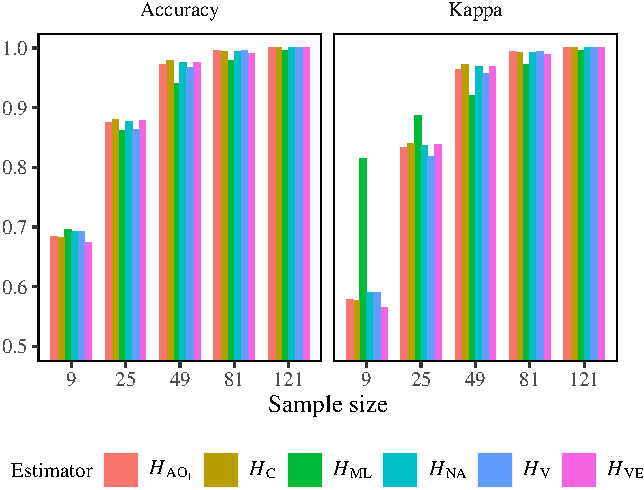
\includegraphics[width=\linewidth]{../../../Figures/CISS2021/measures_samples_synt2.pdf}}
	\subfigure[\label{fig:acc_synt} Using the whole image.]{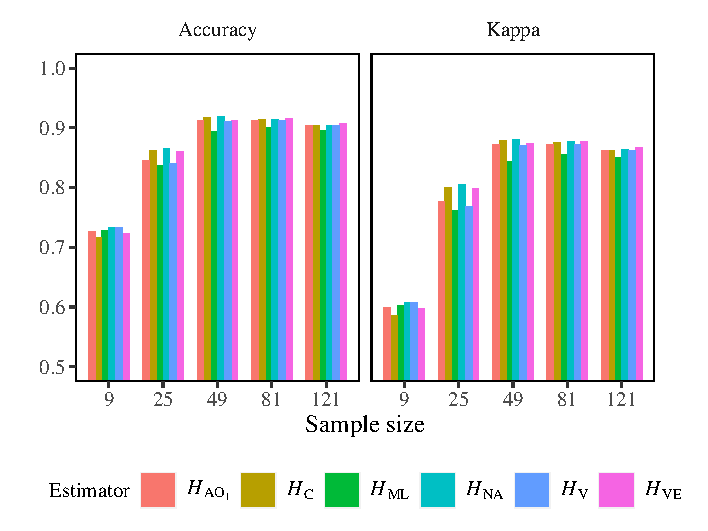
\includegraphics[width=\linewidth]{../../../Figures/CISS2021/measures_synt2.pdf}}
	\caption{Accuracy and Kappa coefficient for SVM.}
\end{figure}    

%%% JC plot_bars_accuracy_synthetic_Figura5.R

%\begin{table}[htbp]
%  \centering
%  \caption{Accuracy and Kappa coefficient values in synthetic image, $L=2$. \textcolor{cyan}{Creo que debiéramos elegir o la Tabla o las barras.}}
%    \label{tab:acc_kappa_synt}
%    \begin{tabular}{cccccccc}
%    \toprule
%    Index & n     & $H_{{AO}_1}$   & $H_\text{C}$    & $H_{\text{NA}}$  % & $H_\text{V}$    & $H_{\text{VE}}$   & $H_{\text{ML}}$ \\
%    \midrule
%    \multirow{2}[2]{*}{Accuracy} & 81    & 0.912 & \textcolor{red}{0.914} & \textcolor{red}{0.914} & 0.912 & \textcolor{red}{0.915} & 0.900 \\
%          & 121   & 0.904 & 0.904 & 0.904 & 0.904 & 0.907 & 0.896 \\
%    \midrule
%    \multirow{2}[1]{*}{Kappa} & 81    & 0.873 & \textcolor{red}{0.876} & \textcolor{red}{0.877} & 0.873 & \textcolor{red}{0.878} & 0.856 \\
%          & 121   & 0.862 & 0.863 & 0.864 & 0.862 & 0.867 & 0.851 \\
%    \bottomrule
%    \end{tabular}
%\end{table}

It can be seen that the best performance is achieved for sliding windows of size $9 \times 9$ and $H_\text{C}$, $H_{\text{NA}}$ and $H_{\text{VE}}$ estimators with $0.914, \ 0.914 \text{ and } 0.915$ respectively for accuracy values,  and  $0.876, \ 0.877 \text{ and } 0.878$ for Kappa index, when the classifier is applied to the whole image.

Since these estimators and window size are the ones that performed the best in the simulated image, we apply them in the classification of an actual image.

\subsection{Actual image}

We used a subsample of $500 \times 645$ pixels from a fully PolSAR image of $900 \times 1024$ data of California's San Francisco bay area, taken by the NASA/JPL AIRSAR L-band instrument, in intensity format where the number of looks $L=4$. Figure~\ref{TrainingSamples} shows this image.

\begin{figure}[hbt]
	\centering
	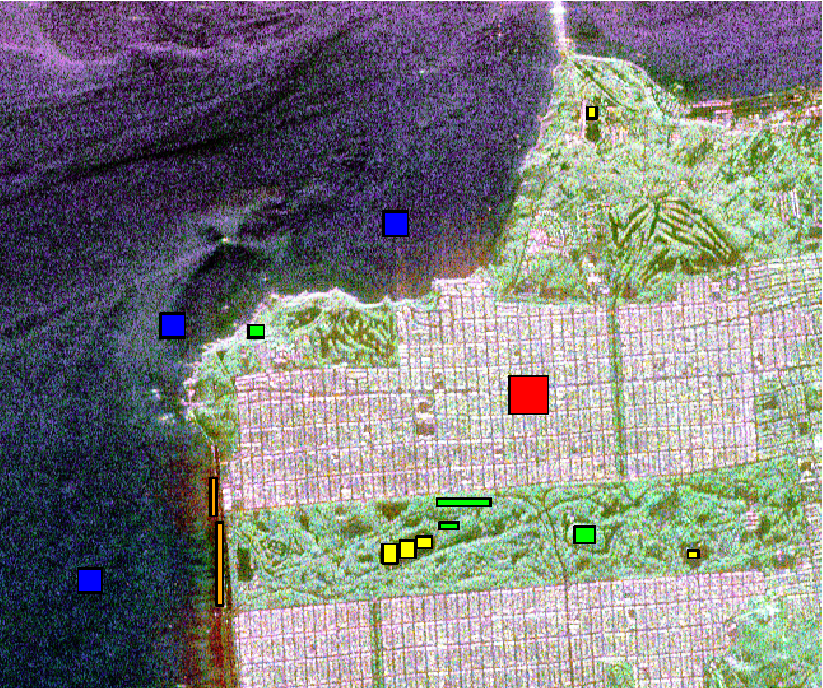
\includegraphics[width=0.9\linewidth]{../../../Figures/CISS2021/muestras_entrenamiento_color2.pdf}
	\caption{Image of San Francisco with reference samples.}
	\label{TrainingSamples}
\end{figure}    

The equivalent number of looks (ENL) using uncorrelated data is defined as
$\text{ENL}={1}/{\widehat{\text{CV}^2}}$, the reciprocal of the sample coefficient of variation $\widehat{\text{CV}}={\widehat{\sigma}}/{\widehat\mu}$, where $\widehat{\sigma}$ is the sample standard deviation and $\widehat\mu$ the sample mean~\cite{Anfinsen2009}. In order to find the ENL in each polarization band, we manually selected samples from homogeneous areas in each band and calculated ENL as an average weighted by the sample size per band. Finally, ENL is the average of the estimations in each polarization. We obtained $2.53, \ 3.41$ and $3.41$ as the ENL values in HH, HV, and VV bands. For these reasons we used the $m$ values for $L=2$, which are the same as $L=3$. 

We applied an SVM algorithm to the image of San Francisco, replicating the procedure described in the study of simulated data, using the entropy estimator as a feature for classification the three polarizations.

Figure~\ref{TrainingSamples} shows the training samples selected to perform the supervised classification. We selected five areas which consist of water (blue), urban zone (red), vegetation (green), pasture (yellow), and beach (orange). 

%\textcolor{blue}{The regions of interests are shown in Figure~\ref{} and %consist of: water (in blue), urban zone (in red), vegetation (in green), %pasture (in yellow) and beach (in orange).
%The sample size is 4217.}

%\textcolor{blue}{We replicated the procedure described in the study of %simulated data, to the image of San Francisco combining the entropy %estimator obtained in each of the three polarizations. 

We studied lineal and radial kernels, but the latter produced the best results with the following hyperparameters:
\begin{itemize}
	\item $c=10$ and $g=1.5$ for $H_\text{C}$,
	\item $c=5$ and $g=2$ for $H_{\text{NA}}$,
	\item $c=10$ and $g=2$ for $H_{\text{VE}}$.
\end{itemize}

We subsequently included the CV as a feature in the classification process, which improved the quality measures. In this case, the best performance is achieved for the linear kernel with a cost of $10$.

Table~\ref{tab:acc_SF} presents the accuracy and Kappa index. 
We can observe that the classification is improved when we consider CV coefficient. In terms of entropy estimators, $H_{\text{NA}}$ seems to be the best classifier, including the CV as a feature.

\begin{table}[htbp]
	\centering
	\caption{Accuracy and Kappa coefficient values in the testing set for the image of San Francisco.}
	\begin{tabular}{lrrrr}
		\toprule
		& \multicolumn{2}{c}{\multirow{2}[-2]{*}{Training with entropy}} & \multicolumn{2}{c}{\multirow{2}[-2]{*}{Training with entropy}} \\
		& \multicolumn{2}{c}{estimators} & \multicolumn{2}{c}{estimators and cv} \\ \cmidrule(lr){2-3}\cmidrule(lr){4-5}          
		& \multicolumn{1}{c}{\textbf{Accuracy}} & \multicolumn{1}{c}{\textbf{Kappa}} & \multicolumn{1}{c}{\textbf{Accuracy}} & \multicolumn{1}{c}{\textbf{Kappa}} \\
		\cmidrule(lr){2-2}\cmidrule(lr){3-3}\cmidrule(lr){4-4}\cmidrule(lr){5-5}
		$H_\text{C}$    & 0.9681 & 0.9596 & 0.9917 & 0.9895 \\
		$H_{\text{NA}}$   & 0.9669 & 0.9581 & 0.9929 & 0.9910 \\
		$H_{\text{VE}}$   & 0.9705 & 0.9626 & 0.9906 & 0.9880 \\
		\bottomrule
	\end{tabular}%
	\label{tab:acc_SF}%
\end{table}%

Figure~\ref{fig:class_SF} exhibits the classification of the whole image of San Francisco when our proposal is applied. It can be observed that the classifier distinguishes the beach and, with the addition of the CV, some roads surrounded by trees are better classified.

\begin{figure}[hbt]
	\centering
	\subfigure[\label{SF_HC} Using $H_\text{C}$.]{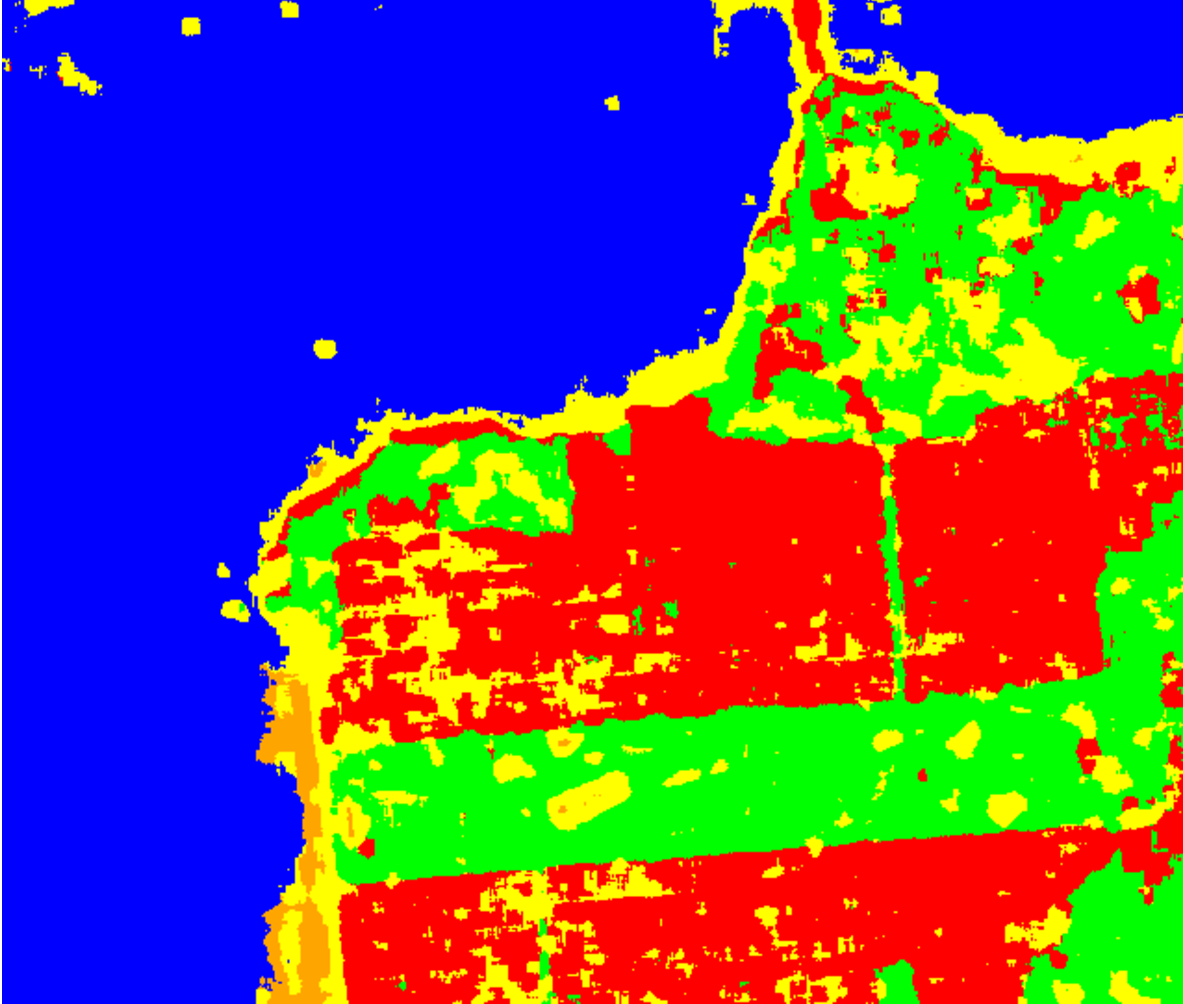
\includegraphics[width=0.45\linewidth]{../../../Figures/CISS2021/SF_HC.pdf}}
	\subfigure[\label{SF_HC_cv} Using $H_{\text{C}}$ and cv.]{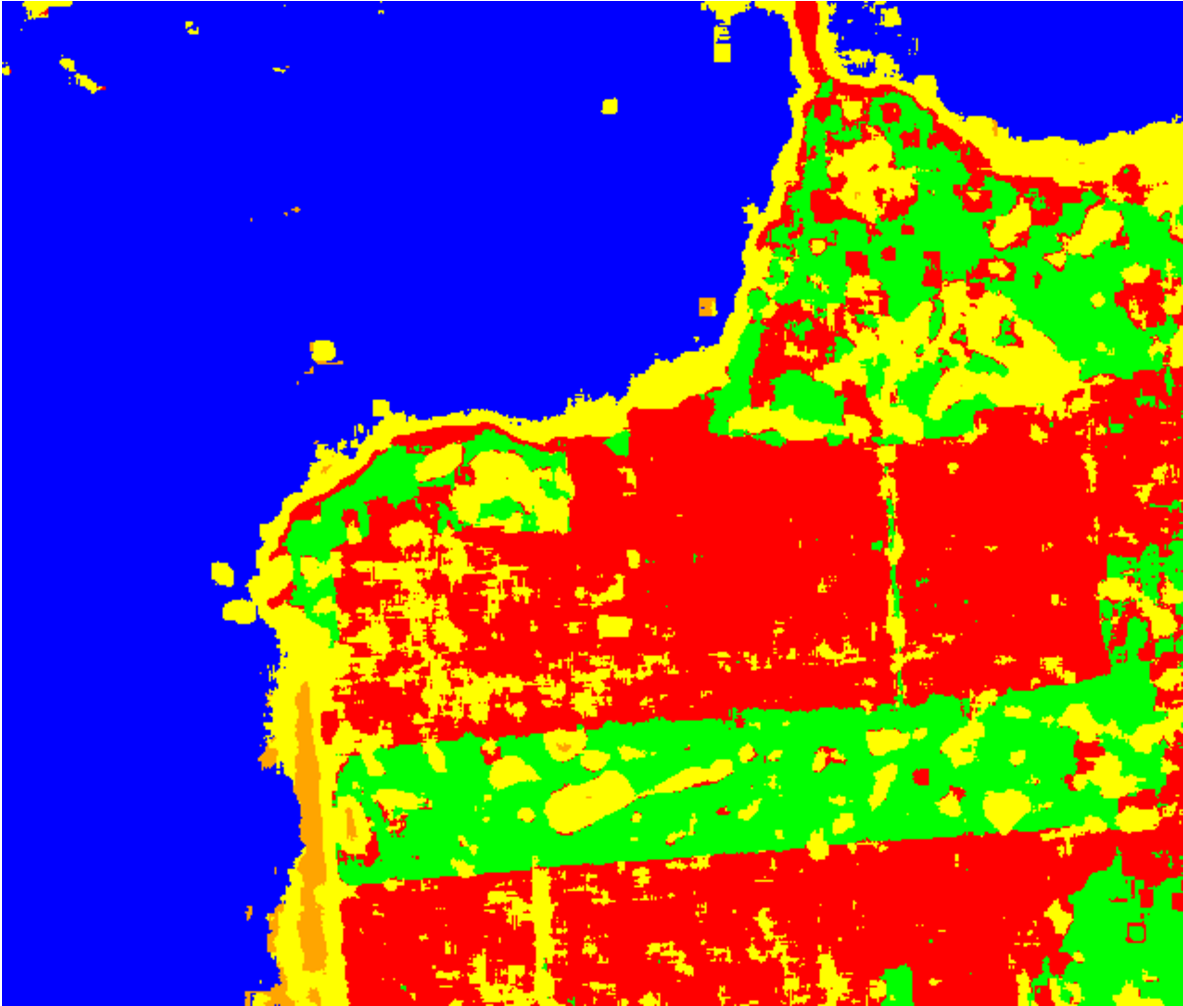
\includegraphics[width=0.45\linewidth]{../../../Figures/CISS2021/SF_HC_cv.pdf}}
	
	\subfigure[\label{SF_HNA} Using $H_{\text{NA}}$.]{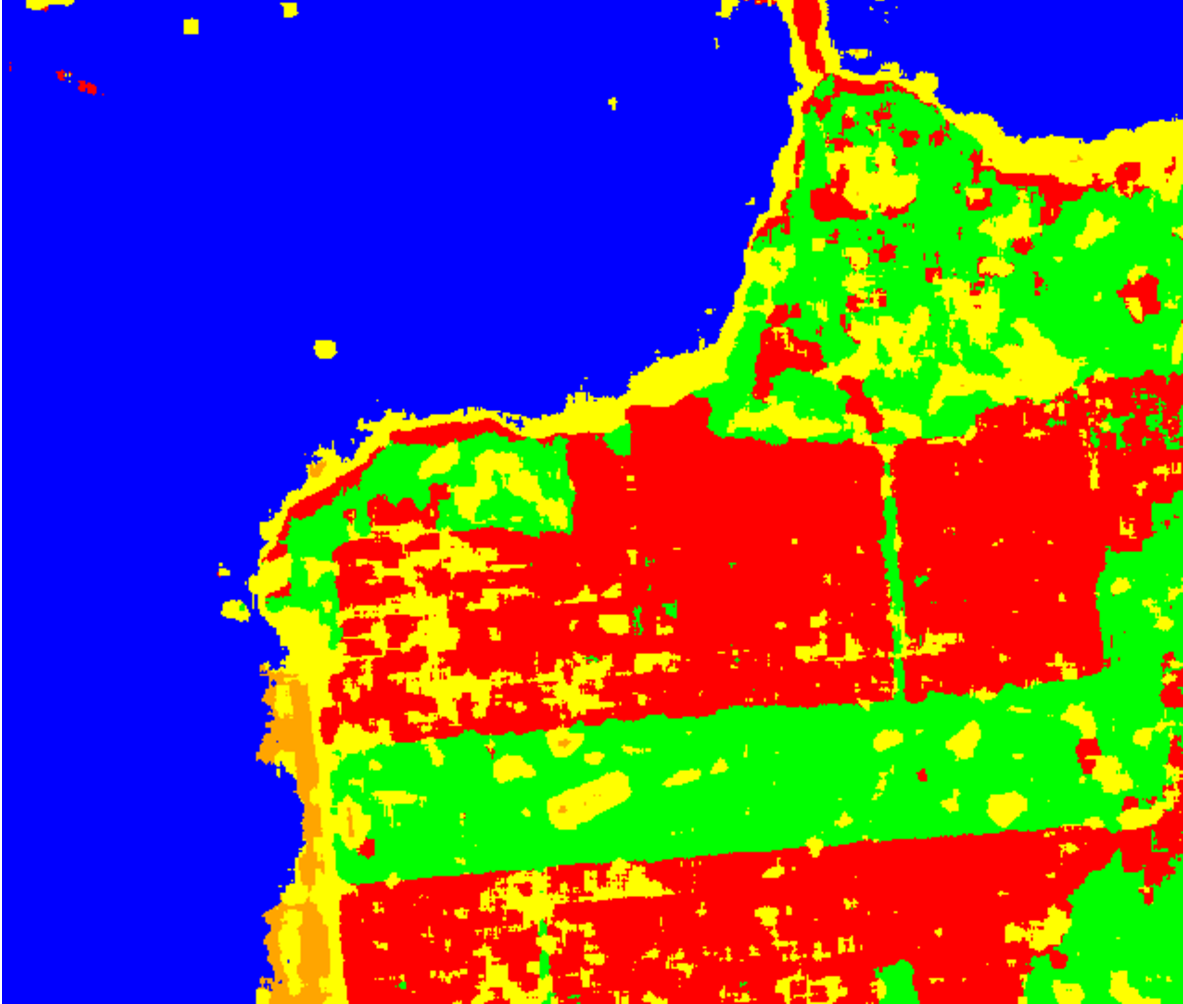
\includegraphics[width=0.45\linewidth]{../../../Figures/CISS2021/SF_HNA.pdf}}
	\subfigure[\label{SF_HNA_cv} Using $H_{\text{NA}}$ and cv.]{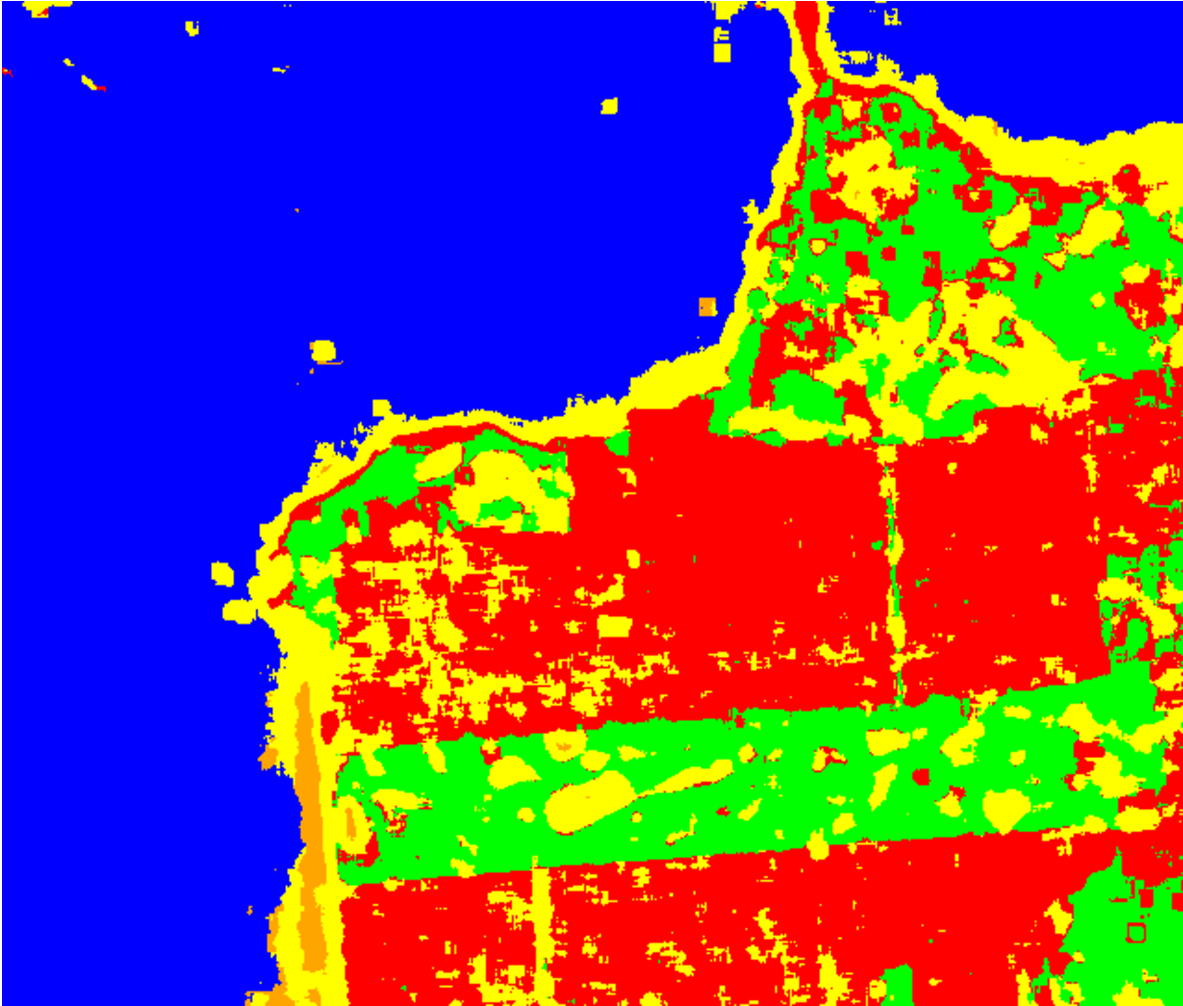
\includegraphics[width=0.45\linewidth]{../../../Figures/CISS2021/SF_HNA_cv.pdf}}
	
	\subfigure[\label{SF_HVE} Using $H_{\text{VE}}$.]{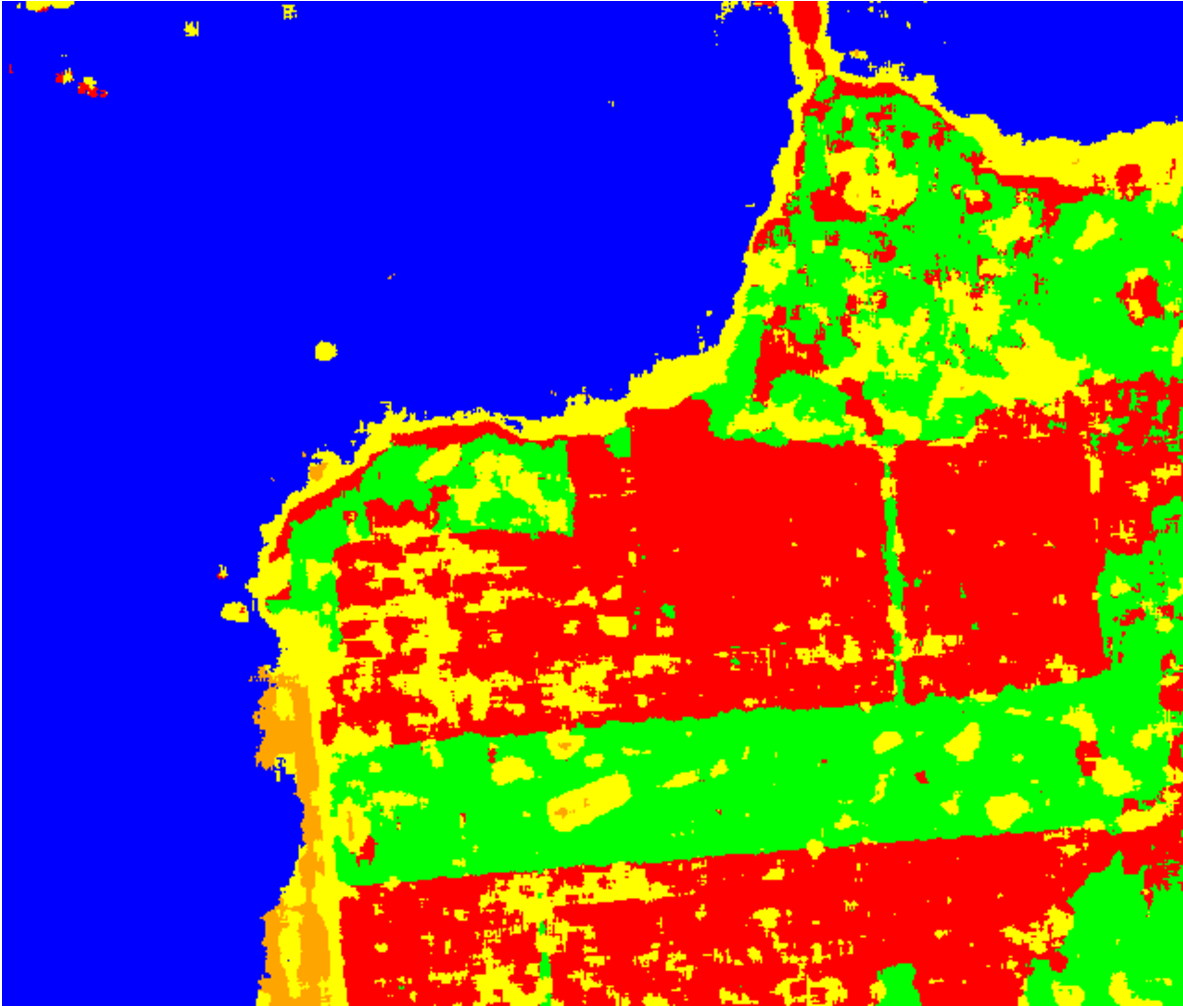
\includegraphics[width=0.45\linewidth]{../../../Figures/CISS2021/SF_HVE.pdf}}
	\subfigure[\label{SF_HVE_cv} Using $H_{\text{VE}}$ and cv.]{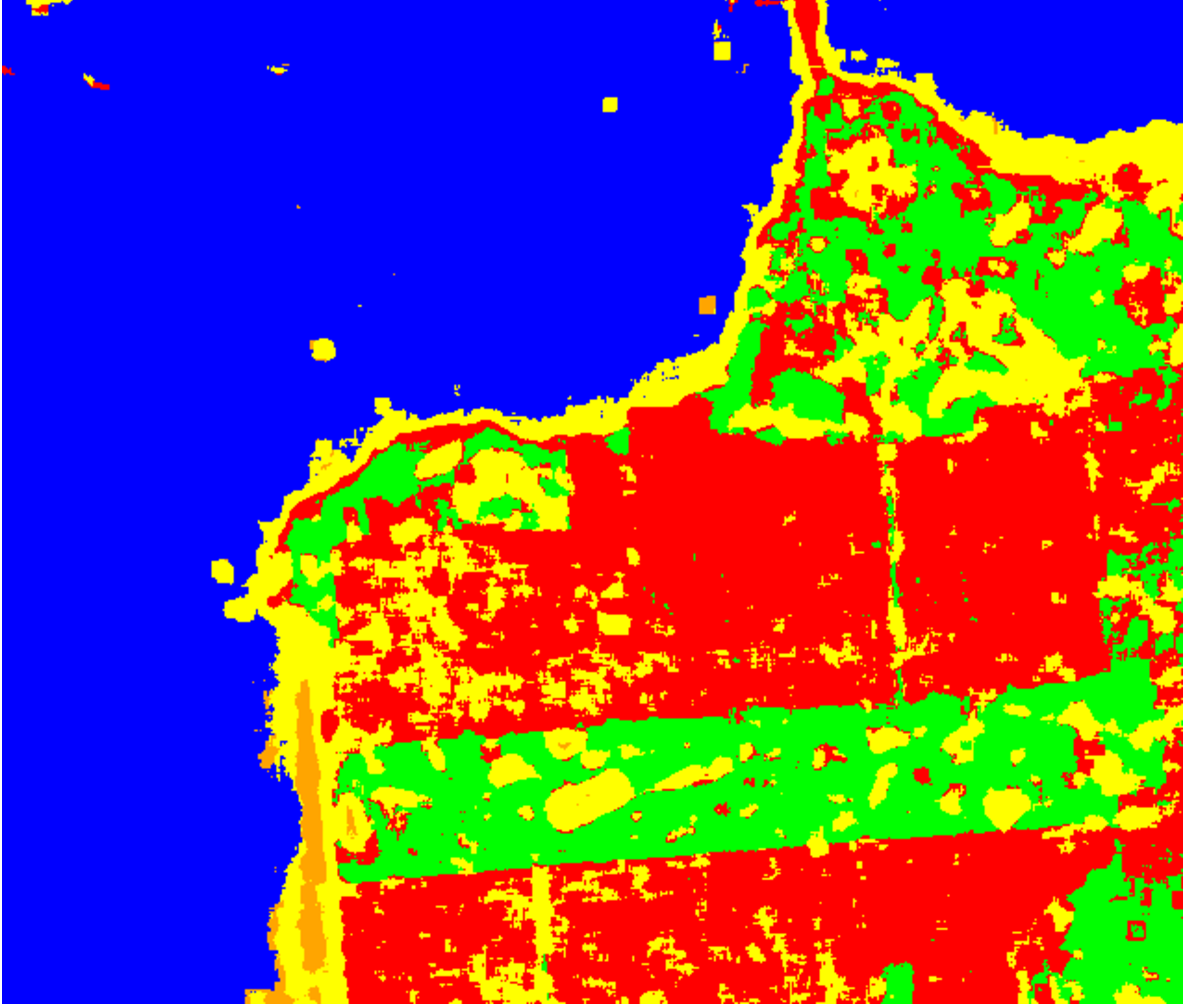
\includegraphics[width=0.45\linewidth]{../../../Figures/CISS2021/SF_HVE_cv.pdf}}
	\caption{San Francisco classification.}
	\label{fig:class_SF}
\end{figure}    

\section{Conclusions}
\label{sec:conclusions}

We assess the performance of six nonparametric entropy estimators in conjunction with the ML estimator in terms of bias and MSE and image classification. 

The advantage of using these nonparametric estimators is that they are very simple to implement. They do not assume any model and do not need to use an optimization algorithm. The disadvantage is that they depend on a spaced parameter $m$. We solved this issue by defining a criterion for choosing the best $m$ that presents the slightest bias in the entropy estimation for all the textured values studied and all sample sizes analyzed. This criterion presents better performance than that of Wieczorkowski et al.~\cite{Wieczorkowski1999}.

With these $m$ values we implemented an unsupervised ($k$-means) and supervised (SVM) classification  algorithm in simulated and actual images and compared their performance with the ML entropy estimator $H_{\text{ML}}$. We displayed that $H_\text{C}$, $H_{\text{NA}}$ and $H_{\text{VE}}$ show the best performance on most of the classification measures used. 

For these estimators, we study their performance applying a supervised classification to a real image. We concluded that $H_{\text{VE}}$ presents the best accuracy an Kappa values, \SI{97}{\percent} and \SI{96}{\percent} respectively. 
% value that present the least bias in the entropy estimation for all the textured values studied and all $n$ value analyzed

In addition, we also considered a new feature, the CV coefficient. We found that both accuracy and Kappa index improved by \SI{2}{\percent}, and that the $H_{\text{NA}}$ estimator presented the best behavior for the studied measures.

\section{Computational information}
\label{conclusion}

All studies were made in the \texttt R platform and language for statistical computing~\cite{RLanguage} (version~4.0.4).

\bibliography{../../../Bibliography/bib_julia2.bib}
\bibliographystyle{IEEEtran}

\begin{IEEEbiography}[{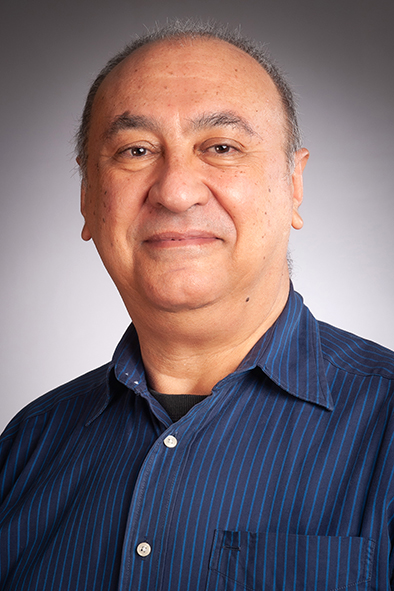
\includegraphics[width=1in,height=1.25in,clip,keepaspectratio]{../../../Figures/Common/ACFreryVUW.jpg}}]{Alejandro C.\ Frery}(S'92--SM'03)
	received a B.Sc. degree in Electronic and Electrical Engineering from the Universidad de Mendoza, Mendoza, Argentina.
	His M.Sc. degree was in Applied Mathematics (Statistics) from the Instituto de Matem\'atica Pura e Aplicada (IMPA, Rio de Janeiro) and his Ph.D. degree was in Applied Computing from the Instituto Nacional de Pesquisas Espaciais (INPE, S\~ao Jos\'e dos Campos, Brazil).
	He is Professor with the School of Mathematics and Statistics, Victoria University of Wellington, New Zealand.
	His research interests are statistical computing and stochastic modeling.
\end{IEEEbiography}

\end{document}